 
\documentclass{beamer}
\setbeamertemplate{section in toc}[sections numbered]
\usefonttheme[onlymath]{serif}
\beamertemplatenavigationsymbolsempty
\setbeamertemplate{footline}{% 
  \hfill% 
  \usebeamercolor[gray!50]{page number in head/foot}% 
  \usebeamerfont{page number in head/foot}% 
  \insertframenumber\,/\,\inserttotalframenumber%
}
\usepackage{amsmath}
\usepackage{graphicx}
% \usepackage{caption}
% \usepackage[skip=0pt]{subcaption}
% \usepackage[tight,FIGTOPCAP]{subfigure}
\usepackage{lmodern}
\usepackage[round]{natbib}
\usepackage{braket}
\usepackage{color}
\usepackage{bm}
\usepackage{amssymb}
\usepackage{bbold}
\usepackage{tikz}
\usepackage{empheq}
\usepackage{stackengine}
\usepackage{framed}
\usepackage[percent]{overpic}
\usepackage{adjustbox}
\DeclareMathOperator{\sgn}{sgn}
\tikzset{>=latex}
\newcommand{\blue}[1]{{\color{blue}{#1}}}
\newcommand{\md}{\mathrm{d}}
\newcommand{\ms}{\mathsf}
\newcommand{\bs}{\boldsymbol}
\newcommand{\mc}{\mathcal}
\renewcommand{\(}{\left(}
\renewcommand{\)}{\right)}
\renewcommand{\[}{\left[}
\renewcommand{\]}{\right]}

%Information to be included in the title page:
\title{Toric Code}
%\author{Apoorv Tiwar, Ammar Jahin, and Yuxuan Wang}
%\institute{University of Florida}
\date{University of Florida, \today}

\begin{document}
\frame{\titlepage} 
\AtBeginSection[]
{
\begin{frame}
    \frametitle{Outline}
    \tableofcontents[currentsection]
\end{frame}
}



\begin{frame}
    \frametitle{Recap of last time}

    \begin{itemize}
        \item The toric code: \begin{align*}
            \mc C = \text{span}\{\ket{\Omega_0} \in \mc H : A(\bm R_i)\ket{\Omega_0} = \ket{\Omega_0}, B(\bm R_i)\ket{\Omega_0} = \ket{\Omega_0} \}
            \end{align*}
        \item A \emph{physical} (local) Hamiltonian can have the codeword space as its ground state: $H = -\sum_{\bm R_i} \(A(\bm R_i)  + B(\bm R_i) \)$.
        \item On a torus, the toric code encode 2 qubits. 
        \item The 2 qubits are manipulated using the non-local operators $Z_1, Z_2. X_1, X_2$. 
        \item The toric codes has an $e^{-\alpha N}$ probability of making an error. 
        \item The toric code is said to store the information encoded in the 2 qubits non-locally. 
        \item Excited states: $S^z(t)\ket{\Omega_0}$ and $S^x(t)\ket{\Omega_0}$. (Open strings.)
        \item The end of open strings can be thought of as particles. The toric code have an $x$-type particle and a $z$-type particle.  
    \end{itemize}

\end{frame}

\section{Anyonic nature of the excitations}
\begin{frame}
    \frametitle{The toric code in different geomtries}
    A (surprising) aspect about the toric code is that the ground state degeneracy depends on the genus, $g$, of the manifold. The toric code is $4^g$ degenerate. 
    
    \pause
    On a \emph{sphere} there are no non-contractible loops. $A(\bm R_i)$ and $B(\bm R_i)$ can label the entire Hilbert space. 
    \begin{columns}
        \begin{column}{0.5\textwidth}
            \begin{itemize}
                \item Hilbert space is $2^{12N^2}$ dimensional.
                \item $6N^2 \ B(\bm R_i)$ operators.
                \item $6N^2 + 2 \ A(\bm R_i)$ operators.
            \end{itemize}
        \end{column}
        \begin{column}{0.5\textwidth}
            \centering
            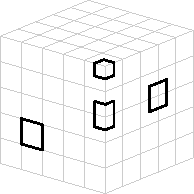
\includegraphics[scale=1.1]{toric_on_sphere.pdf}
        \end{column}
    \end{columns}
    \pause
    \begin{framed}
        The dependance of the ground state degeneracy on the geometry of the manifold is one of the defining features of topological order. 
    \end{framed}
\end{frame}
\begin{frame}
    \frametitle{Particle content of the toric code}
    \begin{columns}
        \begin{column}{0.85\textwidth}
            \begin{itemize}
                \item No particles, 1.
                \item $z$-type particle, referred to as electric charge, $e$.
                \item $x$-type particle, referred to as a magnetic vortex, $m$.
                \item A combinations of an $e$ and an $m$ particle, $\psi = e \times m$
                \item For convince we drop the lattice from the background, and distinguish different strings by different colors.
            \end{itemize}
        \end{column}
    \begin{column}{0.15\textwidth}
        \centering
        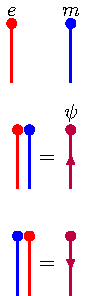
\includegraphics[scale=1]{kinds_of_particles.pdf}
    \end{column}
    \end{columns}
    \pause
    \vspace{10pt}
    Next we ask what are the statistics of these particles. 

    That is we ask What happen when we exchange two $e$, $m$ or $\psi$ particles. 
\end{frame}
\begin{frame}
    \frametitle{A braid group}
    \begin{framed}
        To answer the question about statistics we consider processes that physically exchange the two particles and see how the wavefunction changes under such processes. 
    \end{framed}
    \pause
    \begin{itemize}
        \item It's natural to consider a braid group because of the strings attached to the particles.
        \item There are two kinds of strings. The group is then said to be a colored braid group. 
        \item A state with $2n_e$, and $2n_m$ of $e$ and $m$ particles has $n_e$, and $n_m$ red and blue strings. 
        \item Strings can go above or under each other depending on which operator act first. 
    \end{itemize}
    \centering
    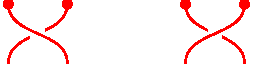
\includegraphics[]{above_under.pdf}
\end{frame}
\begin{frame}
    \frametitle{Brading and fusion rules}
    \begin{columns}
        \begin{column}{0.6\textwidth}
            \begin{itemize}
                \item The electric charge, $e$ is a boson. 
                \item The magnetic vortex, $m$ is a boson. 
                \item $e$ going around $m$ gives a $-1$. 
                \item These phases can be explained as Aharonov-Bohm effect
                \item $\psi$ is a fermion.
            \end{itemize}
        \end{column}
        \begin{column}{0.4\textwidth}
            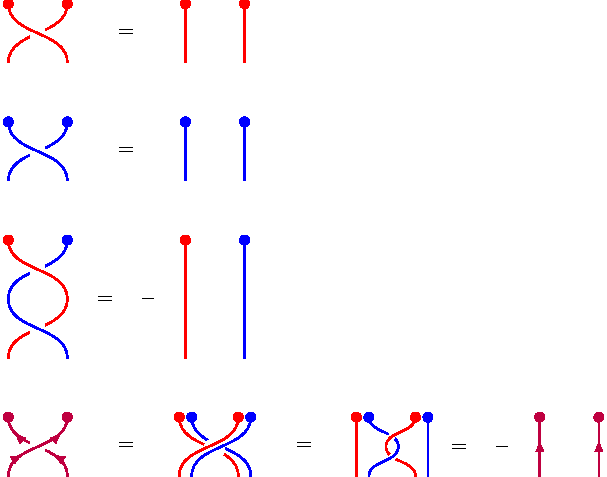
\includegraphics[scale=0.9, trim=0 60 170 0, clip]{rules_of_braiding.pdf}
        \end{column}
    \end{columns}
    \vspace{10pt}
    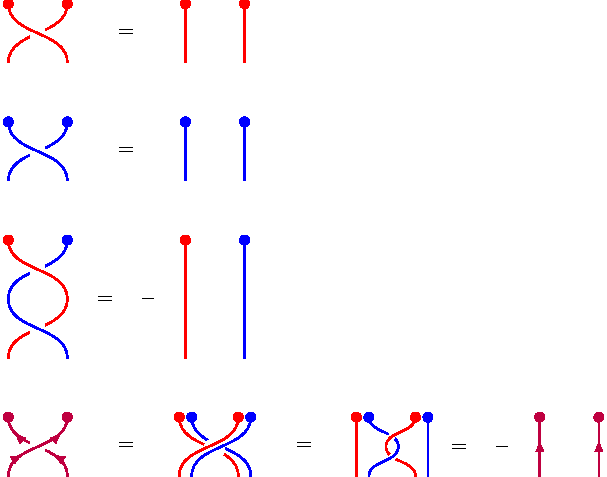
\includegraphics[scale=1, trim=0 0 0 190, clip]{rules_of_braiding.pdf}
\end{frame}

\begin{frame}
    \frametitle{Anyons front and center}
    \framesubtitle{Anyons implies the ground state degeneracy.}

    \begin{framed}
        We can think of the how the anyons braid, as defining the topological order in the system.
    \end{framed}
    \begin{itemize}
        % \item Let $Z_{i}\ (X_{i})$ be the operation that create an $m\ (e)$ particle pair, take one of them around one of the non-contractible loops of the torus, and annihilate the pair again. 
        \item The ground state(s) is a sate with no particles in it. If $\ket{\Omega_0}$ is a ground state, so are $Z_i \ket{\Omega_0}$ and $X_i \ket{\Omega_0}$.
    \end{itemize}
    \begin{itemize}
        \item Braiding rules implies \begin{enumerate}
            \item $Z^2_1 = Z^2_2 = X^2_1 = X^2_2 = 1$
            \item $\[Z_1, Z_2 \] = \[X_1, X_2 \] = 0$
            \item $\{Z_1, X_1 \} = \{Z_2, X_2 \} = 0$.
        \end{enumerate}
        \item This implies the ground state is fourfold degenerate. 
    \end{itemize}
    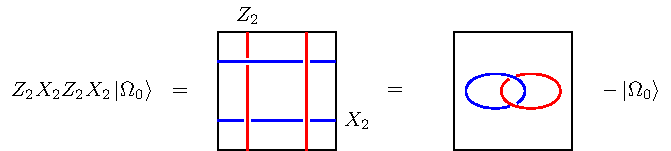
\includegraphics[scale=0.9]{anyons_ground_state.pdf}
    
    
\end{frame}

\begin{frame}
    \frametitle{Summary}

    \begin{itemize}
        \item Quantum codes encode $k$ qubits into $n$ qubits. 
        \item Quantum codes allow for error correction 
        \item The Kitaev toric code encode $2g$ qubits into a spin lattice.  
        \item The Kitaev code has $e^{-\alpha N}$ probability of missing errors. 
        \item Toric code encodes the information non-locally. 
        \item The anyon content of a theory is enough to define its topological order.
    \end{itemize}

\end{frame}


\bibliographystyle{plainnat}
\bibliography{reference}
\end{document} 
 
